\documentclass[11pt]{article}

\usepackage{graphicx}
\usepackage[top=25mm, bottom=25mm, left=25mm, right=25mm, a4paper]{geometry}
\usepackage{amsmath}
\usepackage{enumitem}
\usepackage{float}
\usepackage{fancyhdr}
\usepackage{booktabs}
\usepackage{upquote}
\usepackage{tikz}
\usepackage{steinmetz}
\usepackage{mathrsfs}

\pagestyle{fancy}
\fancyhf{}
\fancyhead[R]{Baturay Kafkas - 2240357068 - Electrical \& Electronics Engineering}

\rfoot{\thepage}
\renewcommand{\headrulewidth}{0pt} 
\renewcommand{\footrulewidth}{0pt}
\sloppy

\begin{document}

\begin{center}
\large
\textbf{ELE228 - Programming for Circuits and Systems Preliminary Work 4}
\end{center}

\section{Questions}

\begin{enumerate}[leftmargin=*,label=\textbf{\arabic*.}]

\item Consider the circuit in \textit{Fig. 1}, derive the differential equation describing the input--output characteristics, where $u(t)$ is the input and $y(t)$ is the output.

\item Compute the impulse response of the system. Implement the impulse response $h(t)$ in
MATLAB and plot it against time.

\item Implement the convolution sum in MATLAB. Create an impulse signal and convolve
it with the impulse response $h(t)$. Compare the output with the impulse response signal.

\begin{figure}[h]
    \centering
    
\includegraphics[width=0.35\linewidth]{fig1.png}

    \textit{Figure 1}
\end{figure}

$R=20~\Omega$ and $C=0.5\cdot10^{-3}$~F.
\end{enumerate}

\section{Answers}

\begin{enumerate}[leftmargin=*,label=\textbf{\arabic*.}]

\item From KVL,
\[\frac1C\int_0^ti(\tau)\,d\tau+y(t)=u(t)\]

Differentiate each side with respect to $t$.
\[\frac{i(t)}{C}+y'(t)=u'(t)\implies \boxed{y'(t)+\frac{y(t)}{RC}=u'(t)}\]

For $R=20\:\Omega$ and $C=0.5\cdot10^{-3}\:$ F,
\[\boxed{y'(t)+100{y(t)}=u'(t)}\]
\item The transfer function is given by
\[H(s)=\frac{Y(s)}{U(s)},\]

where $Y(s)=\mathscr{L}\left\{y(t)\right\}$ and $U(s)=\mathscr{L}\left\{u(t)\right\}$. The $s$--domain equivalent resistance of the capacitor: $\frac{2000}s$. From the voltage divider,
\[Y=U\cdot\frac{20}{20+\frac{2000}s}\implies H=\frac{Y}{U}=\frac{s}{s+100}=1-\frac{100}{s+100}\]
\[\implies h(t)=\mathscr L^{-1}\left\{H(s)\right\}=\delta(t)-100e^{-100t}u(t)\]

\newpage

Code:
\vspace{1em}

\hrule
\begin{verbatim}
num = [1 0];
denom = [1 100];

H_tf = tf(num, denom);
figure
impulse(H_tf)
\end{verbatim}
\hrule

\begin{figure}[H]
    \centering
    
\includegraphics[width=0.7\linewidth]{fig2.png}
\end{figure}

\item Code:
\vspace{1em}

\hrule
\begin{verbatim}
hold on
syms s

H_sym = poly2sym(num,s) / poly2sym(denom,s); 
h = ilaplace(H_sym)

t = 0:10e-4:0.06;

delta_t = zeros(size(t));
delta_t(1) = 1;

h_t = delta_t - 100*exp(-100*t);
h_conv = conv(delta_t, h_t);

plot(t, h_conv(1:length(t)), 'xk')
\end{verbatim}
\hrule

\begin{figure}[H]
    \centering
    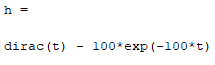
\includegraphics[width=0.4\linewidth]{MATLAB_iMjdF63jju.png}
\end{figure}

\begin{figure}[H]
    \centering
    
\includegraphics[width=0.7\linewidth]{fig3.png}
\end{figure}

The graphs are almost identical. However, because the Dirac delta vector is discrete in MATLAB, the value of the first sample that is convolved is $-99$. Anything else is as anticipated and hence confirms the previous result.

\end{enumerate}

\end{document}